\documentclass[handout]{beamer}
\usepackage{beamerthemesplit}
\usepackage{pgfpages}
\usepackage{verbatim}
\usepackage{amsmath, amssymb, graphics, setspace}

\usepackage{algorithm}
\usepackage{algorithmicx}
\usepackage{algpseudocode}


\newcommand{\field}[1]{\mathbb{#1}} %requires amsfonts

\usetheme{Antibes}
\usecolortheme{beaver}
\title[Thesis Progress Report \#6]{Thesis Progress Report \#6}

\usepackage{mathptmx}
\usepackage[scaled=.90]{helvet}
\usepackage{courier}
\usepackage[T1]{fontenc}

%\pgfpagesuselayout{4 on 1}[letterpaper,border shrink=5mm]

\institute[RIT]{}
\date{\today}
%\subtitle{}
\author{Christopher A. Wood}
%\institute[]{}
\date{\today}

\begin{document}

%%%%%
%%
%% Resource link: http://www.math-linux.com/spip.php?article77
%%
%%%%

\begin{frame}
	\titlepage
\end{frame}

\begin{frame}
	\frametitle{Agenda}
	\tableofcontents
\end{frame}

\section{Decompositions}
\begin{frame}
	\frametitle{Decompositions of Interest}
	\begin{center}
	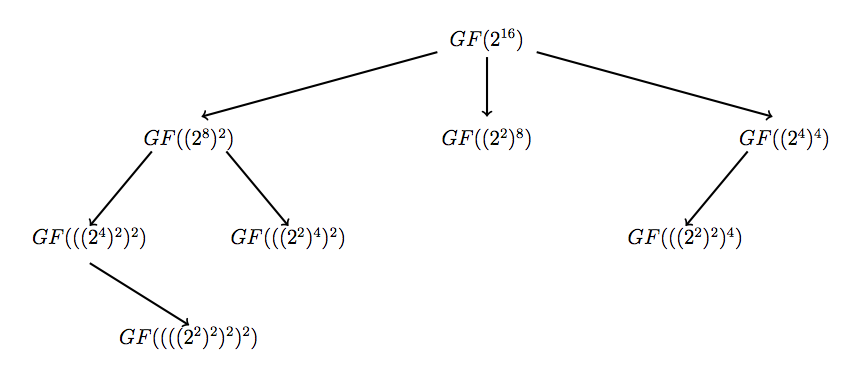
\includegraphics[scale=0.35]{towers.png}
	\end{center}
\end{frame}

\begin{frame}
	\frametitle{Basis Towers for Degree 2 Extensions}
	Let $e(x) = x^2 + x + 1$, $f(x) = x^2 + x + \alpha$, $g(x) = x^2 + x + \lambda$, $\lambda = \alpha^2\beta$

	\medskip 

	Let $e(\alpha) = 0$, $f(\beta) = 0$, $g(\gamma) = 0$
	\begin{itemize}
		\item Satoh - degree 2 extensions with polynomial basis (compactness)
		\begin{itemize}
			\item $e(x) = x^2 + x + 1$ with $\{1, \alpha\}$, $f(x) = x^2 + x + \alpha$ with $\{1, \beta\}$, and $g(x) = x^2 + x + \lambda$ with $\{1, \gamma\}$
		\end{itemize}
		\item Canright - degree 2 extensions with normal basis (compactness)
		\begin{itemize}
			\item $e(x) = x^2 + x + 1$ with $\{\alpha, \alpha^2\}$, $f(x) = x^2 + x + \alpha$ with $\{\beta, \beta^4\}$, and $g(x) = x^2 + x + \lambda$ with $\{\gamma, \gamma^{16}\}$
		\end{itemize}
		\item Nogami - degree 2 extensions with mixed basis (shorter critical path)
		\begin{itemize}
			\item $e(x) = x^2 + x + 1$ with $\{\alpha, \alpha^2\}$, $f(x) = x^2 + x + \alpha$ with $\{1, \beta\}$, and $g(x) = x^2 + x + \lambda$ with $\{\gamma, \gamma^{16}\}$
		\end{itemize}
	\end{itemize}
\end{frame}

\begin{frame}
	\frametitle{Inverse Optimizations}
	With each decomposition, we need an efficient way of computing the multiplicative inverse
	\begin{itemize}
		\item Extended Euclidean algorithm (appropriate for software)
		\item Field decomposition (see slides from reports 1/2) - $n-1$ squarings and $n-2$ multiplications
		\item Fermat's Little theorem: $\alpha^{-1} \equiv \alpha^{2^k - 2}$
		\begin{itemize}
			\item $2^k - 2 = 2 + 2^2 + 2^3 + \dotsb + 2^{k-1}$
			\item $\alpha^{-1} \equiv \alpha^2 \cdot \alpha^{2^2} \cdot \dotsb \cdot \alpha^{2^{k-1}}$
		\end{itemize}
		\item Itoh-Tsujii inversion: $\alpha^{-1} \equiv (\alpha^{r})^{-1}\alpha^{r-1}$, $r = (q^k - 1)/(q-1)$
	\end{itemize}
\end{frame}

\begin{frame}
	\frametitle{Itoh-Tsujii Inversion Algorithm}
\begin{algorithm}[H] 
\caption{Itoh-Tsujii Inversion Algorithm} 
\begin{algorithmic}[1]
\Require{$\alpha \in GF(q^n)$}
\Ensure{$\alpha^{-1} \in GF(q^n)$}
\State $r \gets (q^m - 1)/(q-1)$
\State compute $\alpha^{r-1}$
\State compute $\alpha^r = \alpha^{r-1}\alpha$
\State compute $(\alpha^r)^{-1}$ in $GF(p)$ (base field)
\State compute $\alpha^{-1} = (\alpha^r)^{-1} \cdot \alpha^{r-1}$
\State \Return $\alpha^{-1}$
\end{algorithmic}
\end{algorithm}
\begin{center}
Initially targeted for normal basis to use cyclic shifts for squaring, but can be applied to standard (polynomial) basis as well.
\end{center}
\end{frame}

\section{Basis Change Optimizations}
\begin{frame}
	\frametitle{Optimizing the Basis Change Matrices}
	\begin{itemize}
		\item Paar showed the first greedy approach to final a locally minimum number of `1's in a basis change matrix 
		\item Satoh used this technique to minimize their basis change matrices
		\item Canright implemented optimal tree-search algorithm to minimize the complexity of these matrices
	\end{itemize}
\end{frame}

\section{Hardware and Software}
\begin{frame}
	\frametitle{Hardware and Software}
	\begin{center}
		Demo for polynomial decomposition

		\medskip

		Magma feature review

		\medskip

		VHDL generation
	\end{center}
\end{frame}

\begin{frame}
	\frametitle{Action Items}
	\begin{itemize}
		\item 4th degree inverse decomposition using normal bases
		\item Literature survey on efficient Galois field arithemtic for $GF(2^8)$ - we need optimal squaring, multiplication, and addition operations
		\item Implement 16-bit inverse using normal basis extension of Canright's work
		\item Finish composite field decomposition chapter (overdue)
		\item Outline of code required to perform exhaustive search over all decompositions using all possible bases
	\end{itemize}
	\begin{center}
		Next meeting: \textbf{5/20/13} or \textbf{5/27/13}
	\end{center}
\end{frame}

\end{document}
